\section{Modifying the annotation vocabulary and semantics}

Right-click the project file for which you want to modify the annotation semantics and open it with the \emph{Swproj Model Editor}.
There you can view or edit the EMF model objects that build up a \emph{Reprotool} project. Under the \emph{Software Project} tree node,
you can see the default \emph{Annotation Groups}, what \emph{annotations} and \emph{CTL formulas} they contain. By modifying these
formulas, you can modify the annotation semantics. You can also add new \emph{AnnotationGroups} to add custom annotations to the
\emph{Reprotool} project and to specify their semantics using the NuSMV \emph{CTL formulas}. This paragraph will hopefully make more
sense after you read the programmer's docmentation, especially the chapter on verification.


\begin{figure}[ht]
  \centering
  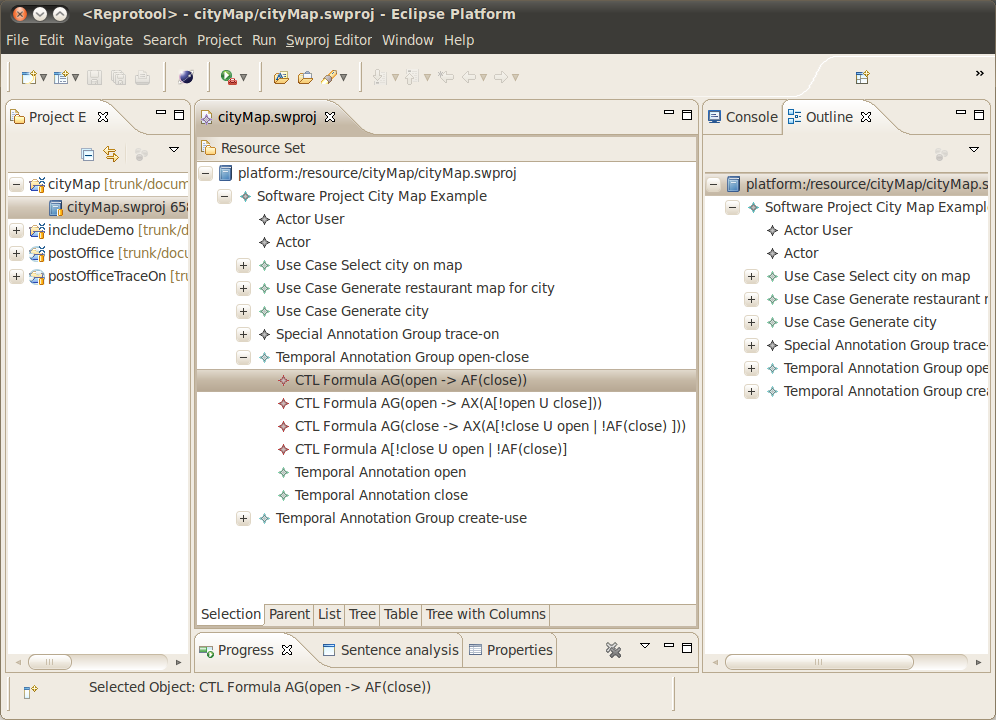
\includegraphics[height=280pt]{images/reprotoolCTLFormulas}
  \caption{The \emph{open-close} annotation group with annotations and default \emph{CTL} formulas}
  \label{fig:reprotoolCTLFormulas}
\end{figure}
